% Author:   Sarah Lawrence
%           sarahy.lawrence@gmail.com 

\documentclass[a4paper,11pt]{article}

\usepackage[T1]{fontenc}
\usepackage[utf8]{inputenc}
\usepackage{graphicx}
\usepackage{xcolor}
\usepackage{graphicx}
\usepackage{subcaption}


\renewcommand\familydefault{\sfdefault}
\usepackage{tgheros}
\usepackage{amsmath,amssymb,amsthm,textcomp}
\usepackage{enumerate}
\usepackage{multicol}
\usepackage{tikz}
\usepackage{courier}

\usepackage{geometry}
\geometry{left=25mm,right=25mm,%
bindingoffset=0mm, top=20mm,bottom=20mm}


\linespread{1.3}

\newcommand{\linia}{\rule{\linewidth}{0.5pt}}

% Titles
\makeatletter
\renewcommand{\maketitle}{
\begin{center}
\vspace{2ex}
{\huge \textsc{\@title}}
\vspace{1ex}
\\
\linia\\
\@author \hfill \@date
\vspace{4ex}
\end{center}
}
\makeatother
%%%

% custom footers and headers
\usepackage{fancyhdr}
\pagestyle{fancy}
\lhead{}
\chead{}
\rhead{Bulldog Game}
\lfoot{Java Swing Experiment}
\cfoot{}
\rfoot{Page \thepage}
\renewcommand{\headrulewidth}{0pt}
\renewcommand{\footrulewidth}{0pt}
%

% code listing settings
\usepackage{listings}
\usepackage{color}

\definecolor{dkgreen}{rgb}{0,0.6,0}
\definecolor{gray}{rgb}{0.5,0.5,0.5}
\definecolor{mauve}{rgb}{0.58,0,0.82}

\lstset{frame=tb,
  language=Java,
  aboveskip=3mm,
  belowskip=3mm,
  showstringspaces=false,
  columns=flexible,
  basicstyle={\small\ttfamily},
  numbers=none,
  numberstyle=\tiny\color{gray},
  keywordstyle=\color{blue},
  commentstyle=\color{dkgreen},
  stringstyle=\color{mauve},
  breaklines=true,
  breakatwhitespace=true,
  tabsize=3
}



% dice set up 
\usepackage{pifont}
\DeclareFontFamily{U}{dice3d}{}
\DeclareFontShape{U}{dice3d}{m}{n}{<-> s*[4] dice3d}{}

%%%----------%%%----------%%%----------%%%----------%%%

\begin{document}

\title{Human and AI Building \\Java Swing Bulldog}

\author{Sarah Lawrence, University of Southern Maine}

\date{02/11/2025}

\maketitle

\section*{Whats the Experiment?}
Can a human with little knowledge of Java Swing work with AI to create a working bulldog user interface? First, what is the game Bulldog? In Bulldog, each turn consists of a player repeatedly rolling a six-sided die until either a 6 is rolled or the player decides to end their turn. If the player rolls a 6, their turn is over, and they score nothing for the turn. The control is then passed on to the next player.
\begin{figure}[h]
    \centering
    \begin{subfigure}{0.45\textwidth}
        \centering
        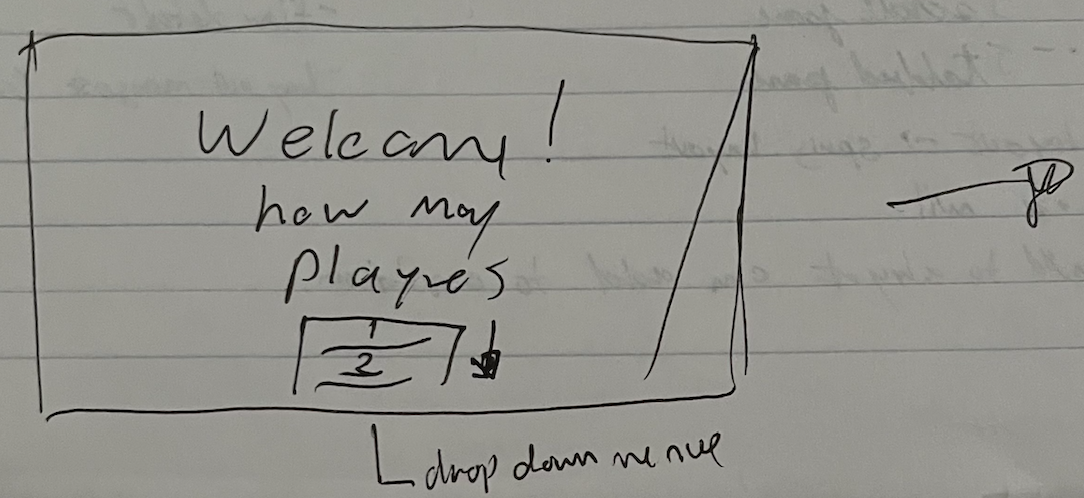
\includegraphics[width=\textwidth]{Image1.png}
        \caption{First Page}
        \label{fig:first}
    \end{subfigure}
    \hfill
    \begin{subfigure}{0.45\textwidth}
        \centering
        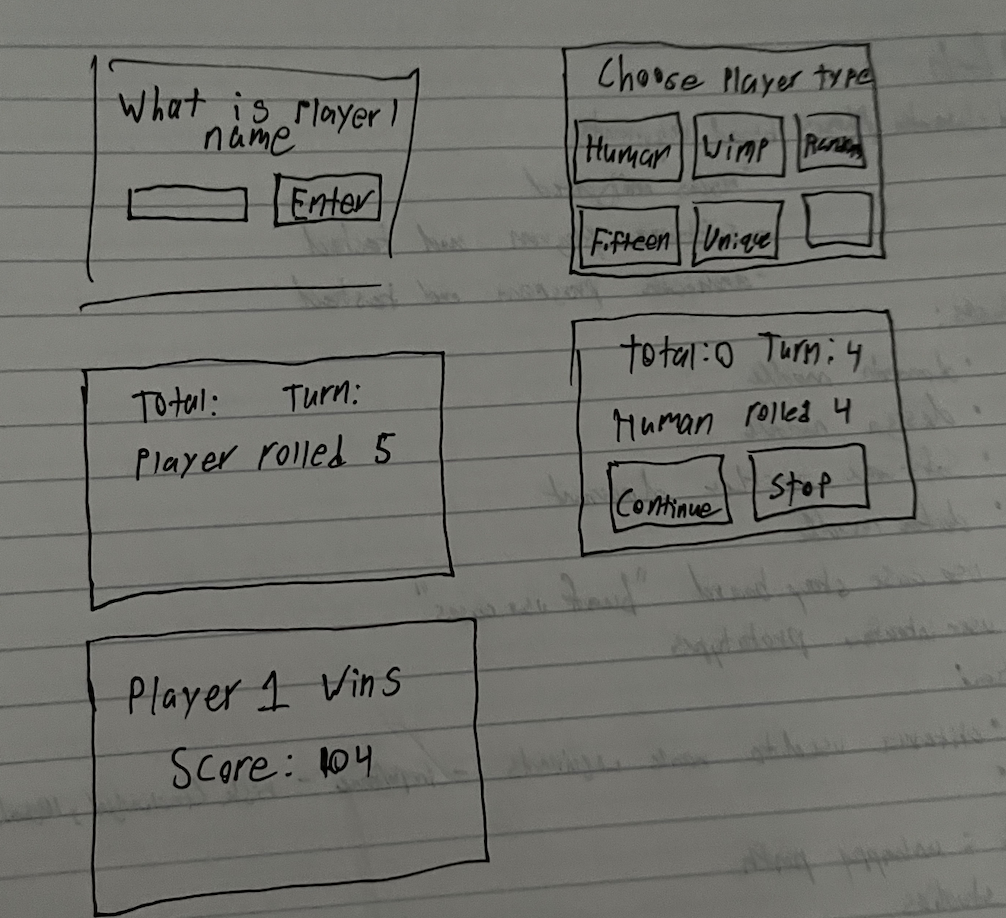
\includegraphics[width=\textwidth]{Image2.png}
        \caption{Second Page}
        \label{fig:second}
    \end{subfigure}
    \caption{The Original Design Sketch \\ Created by: Ashley, Wyatt, and Sarah}
    \label{fig:two_images}
\end{figure}
If a number other than six is rolled, the number is added to the player's turn score. If the player rolls any number other than a 6, the number is added to their score for that turn. If the player wants to continue, they roll the die again, going through the same processes as above. If the player chooses to end their turn, they add their accumulated turn score to their overall score and control passes to the next player. Figure 1 is the initial sketch of the game interface. After Figure 1 it all started with AI prompting.\\
\section*{AI Prompting}
The AI mode used was ChatGBT 5.3 and the whole process took over 20 hours. The prompting approach started simple. Its first goal was to ask if in Java Swing screens transition be possible. This foundation meant that following the design sketch was possible. With this knowledge, the prompts were geared towards making it look like the design sketch. Unfortunately, progress slowly started to unravel when I asked for more complex tasks. Some of those tasks are connecting the player's classes to the functionality of the front. The most challenging task is the last one on the list below.
\subsection*{Prompts Given to the AI}
\begin{itemize}
  \item "In java swing can I have screens transition."
  \item "I want on the first screen to ask the player "Welcome! How many players" and then provide a scroll bar if they pick a number. and have a next page button."
  \item "Scroll pane that has numbers one to five and saves the number the player selects."
  \item "Can i put the numbers in the center of the setSelectionMode"
  \item "Use the selected number to on the second page alow that number of players to types a name. Page layout "what is player 1 name" box [name] [enter] when enter is hit the prompt will change to "what is player 2 name" .."
  \item "On the third page let player one's name pick a player type wimp or random."
  \item "Let both players select a player type."
  \item "Then alow them to go to the next screen where they will have there name above total and turn total and the below what they rolled."
  \item "Not when they end the turn when lets say for example there are two players when both players have rolled the dice and hit end turn then the next round begins change turn to round number and update the number when both players have ended there turns."
  \item "Get rid of round they cant hit next turn untill they hit end turn. next turn should be called next player."
  \item "I end my turn and it still wont let me proceed."
  \item "I end my turn and it still wont let me proceed."
  \item "It breaks it doesn't add the turn score to total and doesn't refresh the turn score how to fix."
\end{itemize}
It was challenging due to how ChatGBT handled it and my lack of knowledge. While working with ChatGBT, when it comes to certain tasks, it often repeats solutions. It performed this looping on the last prompt. I, the programmer having little knowledge of Java Swing, had a hard time discerning and fixing this looping. This lack of familiarity, combined with relying on ChatGBT’s looping, made the experience frustrating. One such thing ChatGBT looped on is it produces code with different variables despite a variable existing doing the same thing. This resulted in the code-breaking and me trying to comb through it to solve the issue. For example:
\subsection*{ChatGBT's Code Explanation}
\begin{verbatim}
Prompt:
"Can I use Player.java when next is clicked so that when turn total gets added to total and then turn total is reset" Player.java is provided with prompt.

Code:
wimpNextTurnButton.addActionListener(e -> {
    // Call the endTurn() method to automatically add the turn total to the score and reset the turn total
    players.get(currentPlayerIndex).endTurn();
    
    // Update the total and turn total labels after the turn ends
    totalLabel.setText("Total: " + players.get(currentPlayerIndex).getScore());
    turnTotalLabel.setText("Turn Total: 0");
\end{verbatim}
The line "players.get(currentPlayerIndex).endTurn();" broke everything. This is because endTurn doesn't exist. What would have worked just fine is adding the turn score to getScore() an already existing method. Coming through to fix problems like these was time-consuming since some of the problems I didn't entirely understand.\\
Overall, it was a painful process. Serval times throughout the project, I considered referring to other documentation to help, but doing so defeated the purpose of the experiment. Unfortunately, the code wasn't any better. 

\section*{Code Description}
The code overall is a mess. ChatGBT had a hard time with the Javadoc style. It kept reverting to its style. It also had a hard time 
when the code got bigger, keeping the organization of the code consistent. Here is an example of some of the inconsistent Javadoc styles. 
\subsection*{Sanple Code}
\begin{lstlisting}
import java.awt.*;
import javax.swing.*;
import java.util.*;

/**
 * A Swing-based game setup with multiple screens for player selection,
 * name entry, player type selection, and the main game screen.
 */
public class ScreenTransitionExample {
    private JFrame frame;
    private JPanel mainPanel;
    private CardLayout cardLayout;
    private JList<Integer> numberList;
    private int selectedNumber = -1; // Number of players
    private ArrayList<String> playerNames = new ArrayList<>();
    private Map<String, String> playerTypes = new HashMap<>();
    private int currentPlayerIndex = 0;

    // Player game data
    private int[] playerScores;
    private int[] playerTurns;
    private int[] turnTotals;  // To track the sum of rolls for the current turn

\end{lstlisting}
However some parts of the code were quite clean and had some of the proper Javadoc styling. \\
For example: 
\begin{lstlisting}
    /**
     * Updates the name prompt for player name entry.
     */
    private void updatePrompt() {
        playerPromptLabel.setText("What is player " + (currentPlayerIndex + 1) + "'s name?");
    }

    /**
     * Updates the type selection prompt for each player.
     */
    private void updateTypePrompt() {
        typePromptLabel.setText(playerNames.get(currentPlayerIndex) + ", choose your type:");
    }
\end{lstlisting}


\section*{Final Result}
Overall the final results could have been better. There is still breaking in some of the player classes. Random doesn't stop rolling if it's just them agents themself. The human player also had problems. The problem is that there is nothing in place to keep the player from rolling the dice. Rolling a 6 will reset the turn total to zero when you hit the end turn, but you can still roll as long as you haven't ended your turn.
Here is what some of it looks like:
\begin{figure}[h]
    \centering
    \begin{subfigure}{0.45\textwidth}
        \centering
        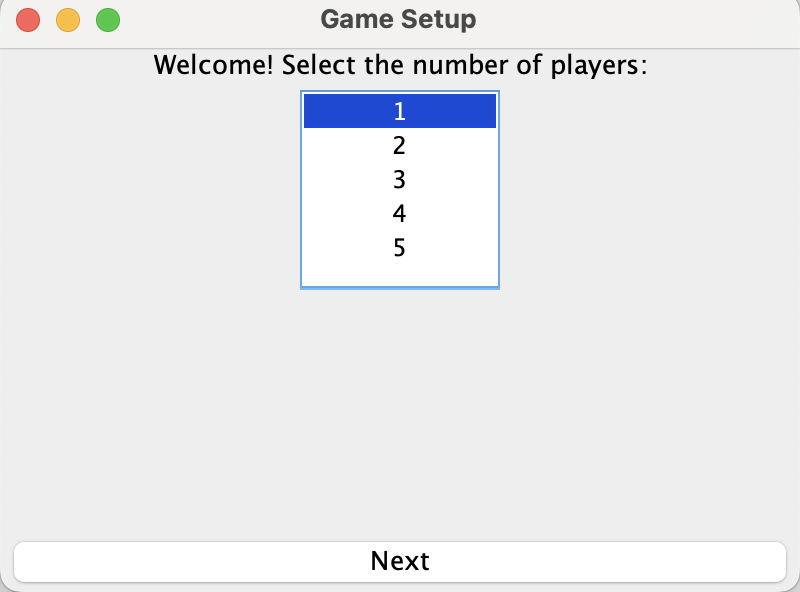
\includegraphics[width=\textwidth]{Image3.png}
        \caption{First Player Screen}
        \label{fig:first}
    \end{subfigure}
    \hfill
    \begin{subfigure}{0.45\textwidth}
        \centering
        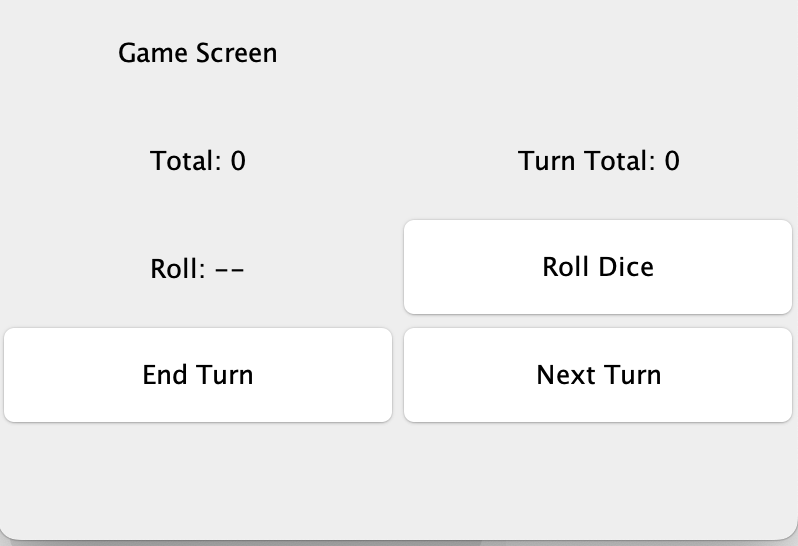
\includegraphics[width=\textwidth]{Image4.png}
        \caption{Final Human Screen}
        \label{fig:second}
    \end{subfigure}
    \caption{Some of the final screens}
    \label{fig:two_images}
\end{figure}

\section*{Conclusion}
All in All, this project was hard and frustrating at times. Not knowing Java Swing hindered my ability to use AI to help. Instead, it became a burden and took me longer to understand. This experience was like working on a group project, but your partner knows more than you. You ask them for help but they have trouble explaining it to you. Then suddenly their stuck and can't figure something out. You try to help but you can't help cause you don't know. That's how the whole project felt for me playing a constant game of catch-up. It was still interesting to see the techniques the AI used. 

\end{document}
